\subsubsection{Temporal Partition Scheduler}
\label{sec:Temporal_Partition_Scheduler}

DREMS components are grouped into processes that are assigned to temporal partitions, implemented by the DREMS OS scheduler. This scheduler was implemented by modifying the behavior of the standard Linux scheduler, introducing an ARINC-653 ~\cite{ARINC-653} style temporal and spatial partitioning scheme. 

\vspace{-0.12in}
\begin{figure}[ht]
\centering
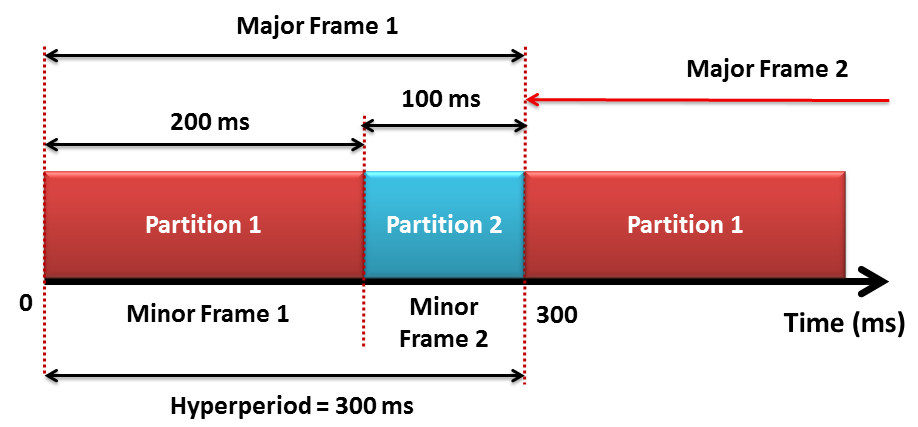
\includegraphics[width=0.37\textwidth]{partition_scheduling}
\caption{Sample Temporal Partition Schedule with Hyperperiod = 300 ms}
\label{fig:partition_scheduling}
\vspace{-0.1in}
\end{figure}


% THis is probablky not needed - the only relevant topic here is temporal partitioning.
%The scheduler further groups threads into different criticality levels: Critical, Application, and Best-Effort. Critical threads handle system and mission management tasks; Application-level threads include component executor threads that perform mission-specific non-critical tasks; Best-Effort threads handle low priority tasks that are scheduled only when there are no other runnable threads from the other two categories.
Temporal partitions are periodic fixed intervals of the CPU's time. Threads associated with a partition are scheduled only when the partition is active. This enforces a temporal isolation between threads assigned to different partitions. The repeating partition windows are called \emph{minor frames}. The aggregate of repeating minor frames is called a \emph{major frame}. The duration of a major frame is called the \emph{hyperperiod}, which is typically the lowest common multiple of the partition periods. Each minor frame is characterized by a period and a duration. The period indicates how often this partition becomes active and the duration indicates how much of the CPU time is available for scheduling the runnable threads associated with that partition. Temporal partitions with fixed periods and durations are chosen such that a valid execution schedule is realized by their coexistence. Figure \ref{fig:partition_scheduling} shows a sample temporal partition schedule. 

%This schedule is made up of two minor frames. Assuming the schedule is enforced at time t = 0, partition 1, characterized by minor frame 1, is made active by the partition scheduler. This partition stays active for the duration of the minor frame, 200 ms. At this point, partition 1 is deactivated and partition 2, characterized by minor frame 2, is activated. Partition 2 stays active for 100 ms, after which the major frame ends and the schedule is repeated.

\subsection{Colored Petri Nets}

Petri nets \cite{Murata1989} are a graphical modeling tool used for describing and analyzing a wide range of systems. A Petri net is a five-tuple $(P, T, A, W, M0)$ where P is a finite set of places, T is a finite set of transitions, A is a finite set of arcs between places and transitions, W is a function assigning weights to arcs, and M0 is the initial marking of the net. Places hold a discrete number of markings called tokens. Tokens often represent resources in the modeled system. A transition can legally fire when all of its input places have necessary number of tokens. 
% Simplify...
%Since Petri net tokens are not distinguishable, the obtained model is often too complex for large systems. To enable compact representations for the modeled system, extensions to the basic Petri net model, called high-level Petri nets, are preferred.
With Colored Petri nets (CPN) \cite{CPN}, tokens contain values of specific data types called colors. Transitions in CPN are enabled for firing only when valid colored tokens are present in all of the typed input places, and valid arc bindings are realized to produce the necessary colored tokens on output places. The firing of transitions in CPN can check for and modify the data values of these colored tokens. Furthermore, large and complex models can be constructed by composing smaller sub-models as CPN allows for hierarchical description. This extended paradigm can more easily model and analyze systems with typed parameters. 

